% ============================================================================
\chapter{실험 및 결과}\label{ch:experiments}
% ============================================================================

이 장은 실험 환경과 평가 방법(\secref{sec:exp_env}--\secref{sec:exp_eval})을 먼저 설명한 뒤, 결과를 가설 순서에
따라 제시한다. H1은 \secref{sec:exp_baseline}, H2는 \secref{sec:sweep}--\secref{sec:exp_lodo},
H3은 \secref{sec:exp_quant}에서 다루고, \secref{sec:exp_final}에서 단계별 누적 결과를 정리한다.

\section{실험 환경}\label{sec:exp_env}

\tabref{tab:env}는 실험에 사용한 하드웨어와 소프트웨어이다. 학습과 GPU 지연 측정은 NVIDIA A100 GPU에서,
CPU 지연 측정은 같은 서버의 CPU에서 수행하였다.

% 자동 생성 파일 — scripts/make_thesis.py 가 덮어쓴다. 직접 고치지 말 것.
\begin{table}[htbp]
\centering
\small
\caption{실험 환경.}
\label{tab:env}
\begin{adjustbox}{max width=\linewidth}
\begin{tabular}{ll}
\toprule
항목 & 사양 \\
\midrule
GPU & NVIDIA A100-SXM4-80GB, 81920 MiB $\times$ 3 \\
CPU & AMD EPYC 9654 96-Core Processor (192 논리 코어) \\
Python / PyTorch / CUDA & 3.10.18 / 2.5.1+cu121 / 12.1 \\
Ultralytics & 8.3.181 (커스텀 패치 적용) \\
ONNX Runtime & 1.23.0 \\
OpenVINO / NNCF & 2026.2.1 / 3.2.0 \\
NumPy / SciPy / OpenCV & 2.1.2 / 1.15.3 / 4.12.0 \\
\bottomrule
\end{tabular}
\end{adjustbox}
\end{table}


\section{학습 설정}\label{sec:exp_train}

모든 모델은 COCO 사전학습 가중치(\texttt{yolo11n-seg.pt}, \texttt{yolo11s-seg.pt})에서 미세 조정하였다.
제안 모델은 제안 구성 파일로 모델을 만든 뒤 같은 사전학습 가중치를 이식하였으며, 새로 추가된 경계 분기만
무작위로 초기화된다. 학습 설정은 \tabref{tab:hparams}와 같다. 옵티마이저는 Ultralytics의 자동 선택에 맡겼으며,
전체 반복 횟수에 따라 AdamW(학습률 0.002, 모멘텀 0.9)가 선택되었다. 최대 100 epoch 동안 학습하되 검증 fitness가
20 epoch 동안 개선되지 않으면 조기 종료하였고, 검증 fitness가 가장 높은 epoch의 가중치를 최종 모델로 사용하였다.
fold별 실제 학습 epoch은 \tabref{tab:epochs}에 있다.

% 자동 생성 파일 — scripts/make_thesis.py 가 덮어쓴다. 직접 고치지 말 것.
\begin{table}[htbp]
\centering
\small
\caption[학습 설정.]{학습 설정. 베이스라인과 제안 모델은 경계 손실 계수를 제외한 모든 값이 같다(생성 시 두 모델의 \texttt{args.yaml}이 일치하는지 자동 확인함).}
\label{tab:hparams}
\begin{adjustbox}{max width=\linewidth}
\begin{tabular}{lp{0.74\linewidth}}
\toprule
구분 & 설정값 \\
\midrule
최적화 & \parbox[t]{0.72\linewidth}{\raggedright \texttt{epochs}=100, \texttt{patience}=20, \texttt{batch}=32, \texttt{imgsz}=640, \texttt{optimizer}=auto, \texttt{lr0}=0.01, \texttt{lrf}=0.01, \texttt{momentum}=0.937, \texttt{weight\_decay}=0.0005, \texttt{warmup\_epochs}=3.0, \texttt{cos\_lr}=False, \texttt{amp}=True} \\
손실 가중치 & \parbox[t]{0.72\linewidth}{\raggedright \texttt{box}=7.5, \texttt{cls}=0.5, \texttt{dfl}=1.5, \texttt{overlap\_mask}=True, \texttt{mask\_ratio}=4} \\
데이터 증강 & \parbox[t]{0.72\linewidth}{\raggedright \texttt{hsv\_h}=0.015, \texttt{hsv\_s}=0.7, \texttt{hsv\_v}=0.4, \texttt{degrees}=0.0, \texttt{translate}=0.1, \texttt{scale}=0.5, \texttt{shear}=0.0, \texttt{perspective}=0.0, \texttt{flipud}=0.0, \texttt{fliplr}=0.5, \texttt{mosaic}=1.0, \texttt{close\_mosaic}=10, \texttt{mixup}=0.0, \texttt{copy\_paste}=0.0} \\
재현성 & \parbox[t]{0.72\linewidth}{\raggedright \texttt{seed}=42, \texttt{deterministic}=True} \\
경계 손실 (제안) & \texttt{head\_gain}=1.0, $\lambda$=2.0 (\ref{sec:sweep}절 스윕으로 결정) \\
\bottomrule
\end{tabular}
\end{adjustbox}
\end{table}


\section{평가 방법}\label{sec:exp_eval}

\subsection{정확도 지표}

\paragraph{Mask \mAP{}.} Ultralytics의 검증 절차로 held-out 집합에서 계산한 마스크 기준 평균 정밀도로,
IoU 임계값 0.50부터 0.95까지 0.05 간격의 10개 임계값에 대한 평균이다.

\paragraph{경계 지표.} 경계 지표는 의미 분할 형태로 계산한다. 신뢰도 0.25 이상, NMS IoU 0.7로 얻은 예측
결절들을 원본 해상도 마스크로 복원하여 합집합 $\bm{P}$를 만들고, 정답 결절 다각형의 합집합 $\bm{G}$와 비교한다.
영상 $I$의 높이·너비를 $h, w$, 대각선 길이를 $D=\sqrt{h^2+w^2}$라 하자.

\begin{itemize}
  \item \textbf{Dice}: $\mathrm{Dice} = 2|\bm{G}\cap\bm{P}| / (|\bm{G}|+|\bm{P}|)$. 두 마스크가 모두 비어 있으면 1로 둔다.
  \item \textbf{HD95}: 마스크와 그 1픽셀 침식의 차로 경계 $\partial\bm{G}, \partial\bm{P}$를 얻고, 거리 변환으로
    한 경계의 각 점에서 다른 경계까지의 거리 $d(\cdot,\cdot)$를 구한다.
    \begin{equation}
      \mathrm{HD95} = \frac{100}{D}\max\Big\{\, P_{95}\big(d(x,\partial\bm{P})\big)_{x\in\partial\bm{G}},\
      P_{95}\big(d(y,\partial\bm{G})\big)_{y\in\partial\bm{P}} \Big\}
      \label{eq:hd95}
    \end{equation}
    $P_{95}$는 95 백분위값이다. 해상도가 영상마다 다르므로 대각선 대비 백분율로 정규화하였다. 예측이나 정답 중
    한쪽의 경계가 없으면 최대 벌점 100\%를 준다.
  \item \textbf{Boundary IoU}\citep{cheng2021boundaryiou}: 폭 $d=\mathrm{round}(0.02D)$의 경계 띠
    $\bm{G}_d = \bm{G} - \ero_d(\bm{G})$, $\bm{P}_d = \bm{P} - \ero_d(\bm{P})$에서 IoU를 구한다.
    \begin{equation}
      \mathrm{BIoU} = \frac{|\bm{G}_d\cap\bm{P}_d|}{|\bm{G}_d\cup\bm{P}_d|}
      \label{eq:biou}
    \end{equation}
    $\ero_d$는 반지름 $d$인 타원형 구조 요소로 침식하는 연산이다.
\end{itemize}

세 경계 지표는 영상마다 계산한 뒤 평균한다. 따라서 결절이 큰 영상이 평균을 지배하지 않는다.

\subsection{효율 지표}

파라미터 수와 640$\times$640 입력 기준 GFLOPs를 보고하고, 지연 시간은 전처리와 후처리(NMS 등)를 제외한
순수 순전파 시간으로 측정하였다. batch 1의 640$\times$640 입력으로 15회 워밍업한 뒤 100회 반복 실행한 평균이다.
ONNX 모델은 ONNX Runtime의 CPU·CUDA 실행 공급자로, OpenVINO 모델은 OpenVINO 런타임의 CPU 장치로 측정하였다.

\subsection{통계 검정}\label{sec:exp_stats}

평균의 차이가 우연의 범위 안인지를 판단하기 위해 세 단위에서 대응표본 검정을 수행하였다.

\begin{itemize}
  \item \textbf{영상 단위 (주 분석).} held-out 614장 각각에 대해, 5개 fold 모델의 지표를 평균한 값을 베이스라인과
    제안 모델 사이에서 짝지어 비교한다. Wilcoxon 부호 순위 검정\citep{wilcoxon1945}(양측)과 대응 $t$ 검정을 함께
    보고하고, 평균 차이의 95\% 신뢰구간을 10,000회 부트스트랩\citep{efron1993bootstrap} 백분위 구간으로 구한다.
  \item \textbf{fold 단위 (보조).} 5개 fold의 평균 지표를 짝지어 비교한다. 학습의 무작위성까지 오차로 포함하는
    보수적인 분석이지만 표본이 5개뿐이어서 검정력이 매우 낮다.
  \item \textbf{시드 단위 (교차 데이터셋).} LODO 실험은 시드 3개(42, 43, 44)의 평균 지표를 대응 $t$ 검정으로 비교한다.
\end{itemize}

효과크기는 대응표본 Cohen's $d_z$\citep{lakens2013effect}, 즉 대응 차이의 평균을 그 표준편차로 나눈 값으로 보고한다.
HD95는 작을수록 좋으므로 부호를 바꾸어, 모든 지표에서 양수가 제안 모델의 우세를 뜻하도록 통일하였다.
'개선 비율'은 대응 차이가 제안 모델 쪽으로 나온 표본의 비율이다.

영상 단위 분석은 테스트 영상의 표본 변동을 오차로 삼으므로 "이 학습 절차로 얻은 모델들이 새 영상에서 더 나은가"에
답한다. 반면 학습 자체의 무작위성은 fold·시드 단위 분석이 반영한다. 두 단위의 결과를 함께 보고하는 이유가
여기에 있으며, 그 해석은 \secref{sec:disc_lodo}에서 다시 다룬다.

\section{기준 모델 선정 (H1)}\label{sec:exp_baseline}

\tabref{tab:nano_small}은 nano와 small을 같은 조건에서 학습하여 held-out 집합에서 비교한 결과이다.

% 자동 생성 파일 — scripts/make_thesis.py 가 덮어쓴다. 직접 고치지 말 것.
\begin{table}[htbp]
\centering
\small
\caption[YOLOv11-seg nano와 small의 비교 (held-out TN3K test, 5-fold 평균 $\pm$ 표준편차).]{YOLOv11-seg nano와 small의 비교 (held-out TN3K test, 5-fold 평균 $\pm$ 표준편차). 굵은 글씨는 더 나은 값이다.}
\label{tab:nano_small}
\begin{adjustbox}{max width=\linewidth}
\begin{tabular}{lcc}
\toprule
지표 & YOLOv11n-seg (nano) & YOLOv11s-seg (small) \\
\midrule
Mask mAP$_{50:95}$ & \textbf{0.6272 $\pm$ 0.0075} & 0.6239 $\pm$ 0.0084 \\
Mask mAP$_{50}$ & \textbf{0.9071 $\pm$ 0.0057} & 0.9067 $\pm$ 0.0073 \\
Box mAP$_{50:95}$ & \textbf{0.6216 $\pm$ 0.0126} & 0.6181 $\pm$ 0.0121 \\
Box mAP$_{50}$ & \textbf{0.9098 $\pm$ 0.0064} & 0.9080 $\pm$ 0.0090 \\
Mask 정밀도 & 0.8757 $\pm$ 0.0182 & \textbf{0.8784 $\pm$ 0.0261} \\
Mask 재현율 & 0.8300 $\pm$ 0.0085 & \textbf{0.8431 $\pm$ 0.0201} \\
\midrule
파라미터 & \textbf{2.84 M} & 10.08 M (3.5배) \\
GFLOPs & \textbf{9.73} & 33.08 (3.4배) \\
가중치 파일 크기 & \textbf{6.00 MB} & 20.51 MB (3.4배) \\
\bottomrule
\end{tabular}
\end{adjustbox}
\end{table}


nano는 Mask \mAP{} 0.6272로 small(0.6239)보다 오히려 근소하게 높았고, Box \mAP{}에서도 0.6216 대 0.6181로
앞섰다. 두 모델의 차이는 모두 fold 표준편차(약 0.008)보다 작아 사실상 같은 수준이다. small은 Mask 재현율이
0.8431로 nano(0.8300)보다 0.013 높았지만 이 역시 small의 fold 표준편차(0.020) 안에 있다. 반면 small은 파라미터
3.5배, 연산량 3.4배, 파일 크기 3.4배를 더 쓴다. 단일 클래스이고 형태 변이가 제한적인 결절 분할에서는 small의
추가 용량이 정확도로 이어지지 않은 것이다. 따라서 \textbf{H1은 지지되며}, 이후 모든 실험은 nano를 기준 모델로 한다.

\section{경계 손실 계수 탐색}\label{sec:sweep}

경계 인식 손실에는 보조 경계 손실 가중치 $g$와 경계 밴드 강조 계수 $\lambda$의 두 계수가 있다
(\eqnref{eq:total_loss}). 처음에는 $g=0.5$, $\lambda=5$로 5개 fold 전체를 학습하였으나, 경계 지표의 개선이 fold마다
엇갈리고 Mask \mAP{}가 0.627에서 0.621로 떨어졌다. 그래서 $g\in\{0.25, 1.0\}$, $\lambda\in\{2, 10\}$의 4개 구성을,
초기값에서 효과의 방향이 갈렸던 fold 0과 2에서 학습하여 비교하였다.

\paragraph{스윕 당시의 선택.} \tabref{tab:sweep_test}는 스윕 모델을 held-out 집합에서 평가한 결과이며, 스윕 당시에는
이 표를 근거로 계수를 골랐다. 다섯 BRM 구성 모두 Dice와 HD95에서 베이스라인보다 나았고, 그중 $g=1.0$, $\lambda=2.0$이
네 지표 모두에서 가장 좋았다. 특히 이 구성만 Mask \mAP{}를 베이스라인 이상(0.6338 대 0.6306)으로 유지하였고,
나머지 구성은 0.010 안팎 낮았다. 이에 따라 $g=1.0$, $\lambda=2.0$을 채택하였다.

% 자동 생성 파일 — scripts/make_thesis.py 가 덮어쓴다. 직접 고치지 말 것.
\begin{table}[htbp]
\centering
\small
\caption[경계 손실 계수 탐색 결과 (fold 0·2 평균, held-out TN3K test 614장).]{경계 손실 계수 탐색 결과 (fold 0·2 평균, held-out TN3K test 614장). $g$는 보조 경계 손실 가중치(\texttt{head\_gain}), $\lambda$는 경계 밴드 강조 계수이며, 굵은 글씨가 채택한 구성이다. 스윕 당시 이 표를 근거로 계수를 선택하였다(\secref{sec:sweep}의 한계 참조).}
\label{tab:sweep_test}
\begin{adjustbox}{max width=\linewidth}
\begin{tabular}{lcccccc}
\toprule
구분 & $g$ & $\lambda$ & Dice$\uparrow$ & HD95 (\%)$\downarrow$ & BIoU$\uparrow$ & Mask mAP$_{50:95}\uparrow$ \\
\midrule
베이스라인 & -- & -- & 0.8132 & 10.835 & 0.4357 & 0.6306 \\
\midrule
초기값 & 0.5 & 5 & 0.8243 & 8.759 (-19.2\%) & 0.4348 & 0.6209 \\
\midrule
스윕 & 0.25 & 2 & 0.8301 & 8.565 (-21.0\%) & 0.4372 & 0.6199 \\
스윕 & 0.25 & 10 & 0.8264 & 8.607 (-20.6\%) & 0.4377 & 0.6203 \\
\textbf{스윕} & \textbf{1} & \textbf{2} & \textbf{0.8368} & \textbf{7.995 (-26.2\%)} & \textbf{0.4473} & \textbf{0.6338} \\
스윕 & 1 & 10 & 0.8258 & 8.378 (-22.7\%) & 0.4318 & 0.6192 \\
\bottomrule
\end{tabular}
\end{adjustbox}
\end{table}


\paragraph{검증 분할을 이용한 사후 점검.} 그러나 평가 집합으로 하이퍼파라미터를 고르면, 선택된 구성의 평가 성능은
선택 과정 자체 때문에 낙관적으로 편향될 수 있다. 이 문제를 확인하기 위해 같은 스윕 모델들을 각 fold의 검증 분할
(학습에 쓰이지 않고 조기 종료에만 쓰인 영상)에서 다시 평가하였다(\tabref{tab:sweep_val}).

% 자동 생성 파일 — scripts/make_thesis.py 가 덮어쓴다. 직접 고치지 말 것.
\begin{table}[htbp]
\centering
\small
\caption[경계 손실 계수 탐색 결과 (fold 0·2 평균, 각 fold의 검증 분할(fold 0: 704장, fold 2: 703장)).]{경계 손실 계수 탐색 결과 (fold 0·2 평균, 각 fold의 검증 분할(fold 0: 704장, fold 2: 703장)). $g$는 보조 경계 손실 가중치(\texttt{head\_gain}), $\lambda$는 경계 밴드 강조 계수이며, 굵은 글씨가 채택한 구성이다. 계수 선택 이후에 같은 모델을 다시 평가한 사후 점검 결과이다.}
\label{tab:sweep_val}
\begin{adjustbox}{max width=\linewidth}
\begin{tabular}{lcccccc}
\toprule
구분 & $g$ & $\lambda$ & Dice$\uparrow$ & HD95 (\%)$\downarrow$ & BIoU$\uparrow$ & Mask mAP$_{50:95}\uparrow$ \\
\midrule
베이스라인 & -- & -- & 0.7954 & 10.574 & 0.3714 & 0.5617 \\
\midrule
초기값 & 0.5 & 5 & 0.8085 & 8.707 (-17.7\%) & 0.3789 & 0.5660 \\
\midrule
스윕 & 0.25 & 2 & 0.8088 & 8.567 (-19.0\%) & 0.3786 & 0.5612 \\
스윕 & 0.25 & 10 & 0.8052 & 9.068 (-14.2\%) & 0.3805 & 0.5649 \\
\textbf{스윕} & \textbf{1} & \textbf{2} & \textbf{0.8041} & \textbf{9.066 (-14.3\%)} & \textbf{0.3798} & \textbf{0.5635} \\
스윕 & 1 & 10 & 0.8057 & 9.137 (-13.6\%) & 0.3769 & 0.5599 \\
\bottomrule
\end{tabular}
\end{adjustbox}
\end{table}


결과는 두 가지로 요약된다. 첫째, \textbf{경계 정교화의 효과 자체는 선택 절차와 무관하게 재현되었다.} 검증 분할에서도
다섯 BRM 구성 모두 베이스라인보다 Dice가 0.009--0.013 높고, HD95가 13.6--19.0\% 낮고, Boundary IoU가 0.006--0.009 높았다.
Mask \mAP{}는 베이스라인과 $\pm$0.005 이내였다. 둘째, \textbf{구성 사이의 순위는 재현되지 않았다.} held-out에서 모든 지표
1위였던 $g=1.0$, $\lambda=2.0$은 검증 분할에서 Dice가 BRM 구성 가운데 가장 낮았고 HD95는 세 번째였으며, 검증 분할에서는
$g=0.25$, $\lambda=2.0$이 Dice와 HD95 모두 가장 좋았다. 다만 검증 분할에서 구성 간 차이(Dice 0.0047, HD95 0.57\%p)는
BRM과 베이스라인의 차이보다 훨씬 작다.

두 결과를 종합하면, $g$와 $\lambda$를 이 범위 안에서 어떻게 고르든 경계 정교화의 이득은 나타나지만, 채택한 구성이
다른 구성보다 특별히 낫다는 근거는 held-out 결과에만 있다. 따라서 \secref{sec:exp_brm}의 최종 개선 폭은 계수 선택 과정의
영향을 받아 실제보다 클 수 있으며, 그 크기는 현재 실험으로 정할 수 없다(\secref{sec:limitations}).
한편 $\lambda=2$가 $\lambda=10$보다 HD95에서 나은 경향은 두 $g$ 값과 두 평가 집합 네 경우 모두에서 일관되었다.
이 현상의 원인은 \secref{sec:disc_lambda}에서 논의한다.

\section{경계 정교화 결과 (H2)}\label{sec:exp_brm}

채택한 계수($g=1.0$, $\lambda=2.0$)로 제안 모델을 5개 fold 전부에서 처음부터 다시 학습하여 베이스라인과 비교하였다
(\tabref{tab:brm_main}, \figref{fig:boundary_improvement}).

% 자동 생성 파일 — scripts/make_thesis.py 가 덮어쓴다. 직접 고치지 말 것.
\begin{table}[htbp]
\centering
\small
\caption[경계 정교화 모듈의 효과 (held-out TN3K test 614장, 5-fold 평균 $\pm$ 표준편차).]{경계 정교화 모듈의 효과 (held-out TN3K test 614장, 5-fold 평균 $\pm$ 표준편차). 마지막 열은 제안 모델이 베이스라인보다 나은 fold 수이다.}
\label{tab:brm_main}
\begin{adjustbox}{max width=\linewidth}
\begin{tabular}{lcccc}
\toprule
지표 & 베이스라인 & 제안 (BRM) & $\Delta$ (상대) & 개선 fold \\
\midrule
Mask mAP$_{50:95}\uparrow$ & 0.6272 $\pm$ 0.0075 & 0.6267 $\pm$ 0.0081 & -0.0005 (-0.1\%) & 2/5 \\
Dice$\uparrow$ & 0.8195 $\pm$ 0.0070 & 0.8300 $\pm$ 0.0039 & +0.0104 (+1.3\%) & 5/5 \\
HD95 (\%)$\downarrow$ & 9.628 $\pm$ 1.175 & 8.378 $\pm$ 0.775 & -1.249 (-13.0\%) & 3/5 \\
Boundary IoU$\uparrow$ & 0.4358 $\pm$ 0.0072 & 0.4414 $\pm$ 0.0050 & +0.0055 (+1.3\%) & 4/5 \\
\midrule
파라미터 & 2,842,803 & 2,847,460 & +4,657 & -- \\
추론 GFLOPs & 9.73 & 9.73 & +0.00 & -- \\
\bottomrule
\end{tabular}
\end{adjustbox}
\end{table}


\begin{figure}[htbp]
  \centering
  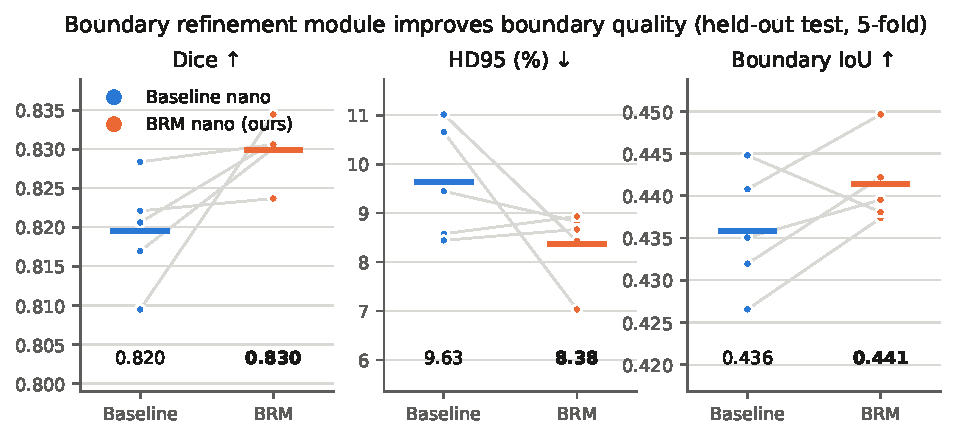
\includegraphics[width=0.92\linewidth]{fig1_boundary_improvement}
  \caption[경계 정교화의 효과 (held-out TN3K test).]{경계 정교화의 효과 (held-out TN3K test). 점은 fold별 값, 회색 선은 같은 fold끼리의 대응,
    가로 막대는 5-fold 평균이다.}
  \label{fig:boundary_improvement}
\end{figure}

세 경계 지표가 모두 개선되었다. Dice는 0.8195에서 0.8300으로 0.0104 올랐고 5개 fold 모두에서 개선되었다.
HD95는 9.628\%에서 8.378\%로 13.0\% 줄었으며, Boundary IoU는 0.4358에서 0.4414로 올랐다(4/5 fold 개선).
fold 간 표준편차도 Dice 0.0070$\rightarrow$0.0039, HD95 1.175$\rightarrow$0.775로 줄어, 제안 모델의 결과가 분할에 덜
민감하였다. HD95는 5개 중 3개 fold에서 개선되었는데, 개선되지 않은 두 fold도 차이가 작았던 반면 개선된 fold의
감소 폭이 커서(\tabref{tab:perfold}) 평균이 크게 줄었다.

Mask \mAP{}는 0.6272에서 0.6267로 사실상 같았다. mAP가 경계 개선을 반영하지 못하는 이유는
\secref{sec:disc_map}에서 논의한다. 추가 파라미터는 4,657개이고 추론 GFLOPs는 9.73으로 같으므로,
경계 개선은 추론 비용 증가 없이 얻은 것이다.

\section{정성적 분석}\label{sec:exp_qual}

\figref{fig:qualitative}는 held-out 영상에서의 예측 경계이다. 개선 폭이 큰 사례만 고르면 그림이 결론을 과장하므로,
무작위로 뽑은 40장 중 결절이 있고 두 모델 모두 예측을 낸 영상을 Dice 개선 폭으로 정렬한 뒤 최상위, 상위 4분위,
중앙값, 최하위에서 한 장씩 골랐다.

\begin{figure}[htbp]
  \centering
  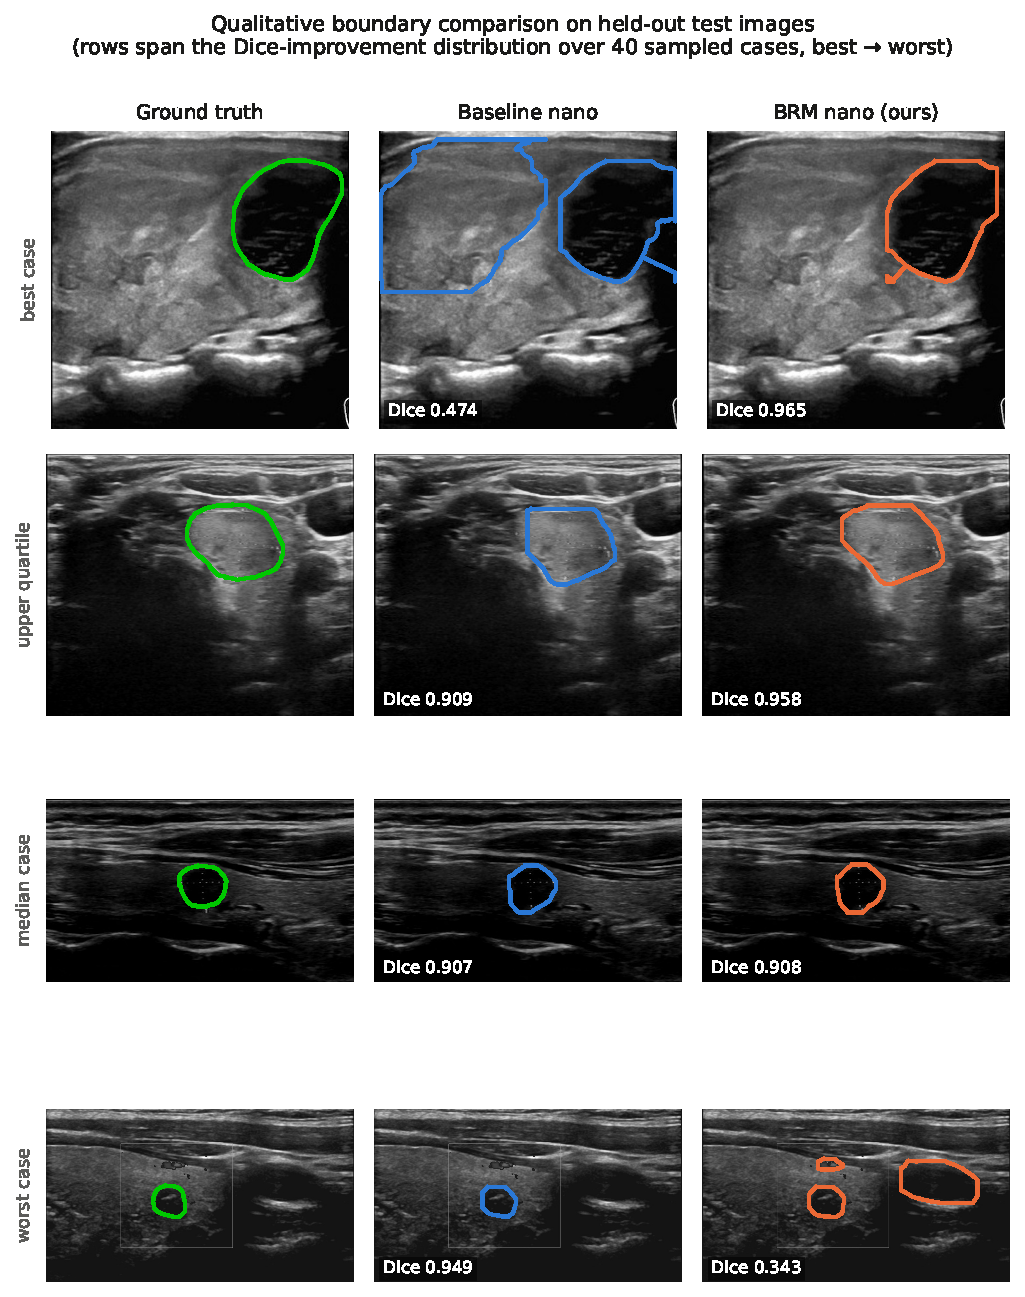
\includegraphics[width=0.72\linewidth]{fig4_qualitative}
  \caption[정성 비교.]{정성 비교. 왼쪽부터 정답 경계, 베이스라인 예측, 제안 모델 예측이며, 행은 위에서부터 Dice 개선 폭의
    최상위·상위 4분위·중앙값·최하위 사례이다. 각 칸의 숫자는 해당 영상의 Dice이다.}
  \label{fig:qualitative}
\end{figure}

상위 사례에서는 제안 모델의 윤곽이 정답에 더 밀착하며, 특히 결절 하방의 음향 음영 구간에서 베이스라인의 경계가
바깥으로 새어 나가는 현상이 줄었다. 중앙값 사례에서는 두 모델의 차이가 거의 없는데, 이는 \secref{sec:exp_sig}의
'개선 비율'이 50\%를 조금 넘는 수준이라는 결과와 일치한다. 최하위 사례는 제안 모델이 결절 옆의 조직을 결절로
함께 포함하여 Dice가 크게 떨어진 경우로, 경계 가중이 잘못 잡힌 경계를 오히려 강화할 수 있음을 보여 주는
실패 유형이다.

\section{통계적 유의성}\label{sec:exp_sig}

\tabref{tab:stats}와 \figref{fig:significance}는 \secref{sec:exp_stats}의 대응표본 검정 결과이다.

% 자동 생성 파일 — scripts/make_thesis.py 가 덮어쓴다. 직접 고치지 말 것.
\begin{table*}[htbp]
\centering
\footnotesize
\caption[경계 정교화 효과의 대응표본 검정 (held-out TN3K test).]{경계 정교화 효과의 대응표본 검정 (held-out TN3K test). 영상 단위 분석은 각 영상에 대해 5개 fold 모델의 예측 지표를 평균한 뒤 비교한다. 95\% 신뢰구간은 대응 차이의 부트스트랩(10,000회) 백분위 구간이며, $d_z$는 대응표본 효과크기로 양수가 제안 모델의 우세를 뜻한다. n=5에서 양측 Wilcoxon 검정이 도달할 수 있는 최소 $p$는 0.0625이다. 대응 $t$ 검정의 $p$는 영상 단위 0.0007, 0.0202, 0.0002, fold 단위 0.071, 0.165, 0.190(Dice, Boundary IoU, HD95 순)로 결론이 같다.}
\label{tab:stats}
\setlength{\tabcolsep}{4pt}
\begin{adjustbox}{max width=\linewidth}
\begin{tabular}{llccccc}
\toprule
분석 단위 & 지표 & $\Delta$ & 95\% CI & Wilcoxon $p$ & $d_z$ & 개선 비율 (\%) \\
\midrule
\multirow{3}{*}{영상 단위 (n=614)} & Dice & +0.0104 & [+0.0044, +0.0166] & $0.014$ (*) & 0.14 & 52.8 \\
 & Boundary IoU & +0.0055 & [+0.0009, +0.0102] & $0.011$ (*) & 0.09 & 53.6 \\
 & HD95 (\%) & -1.2495 & [-1.8945, -0.5918] & $0.0045$ (**) & 0.15 & 53.4 \\
\midrule
\multirow{3}{*}{fold 단위 (n=5)} & Dice & +0.0104 & -- & $0.062$ (n.s.) & 1.09 & 100.0 \\
 & Boundary IoU & +0.0055 & -- & $0.188$ (n.s.) & 0.76 & 80.0 \\
 & HD95 (\%) & -1.2495 & -- & $0.312$ (n.s.) & 0.71 & 60.0 \\
\bottomrule
\end{tabular}
\end{adjustbox}
\end{table*}


\begin{figure}[htbp]
  \centering
  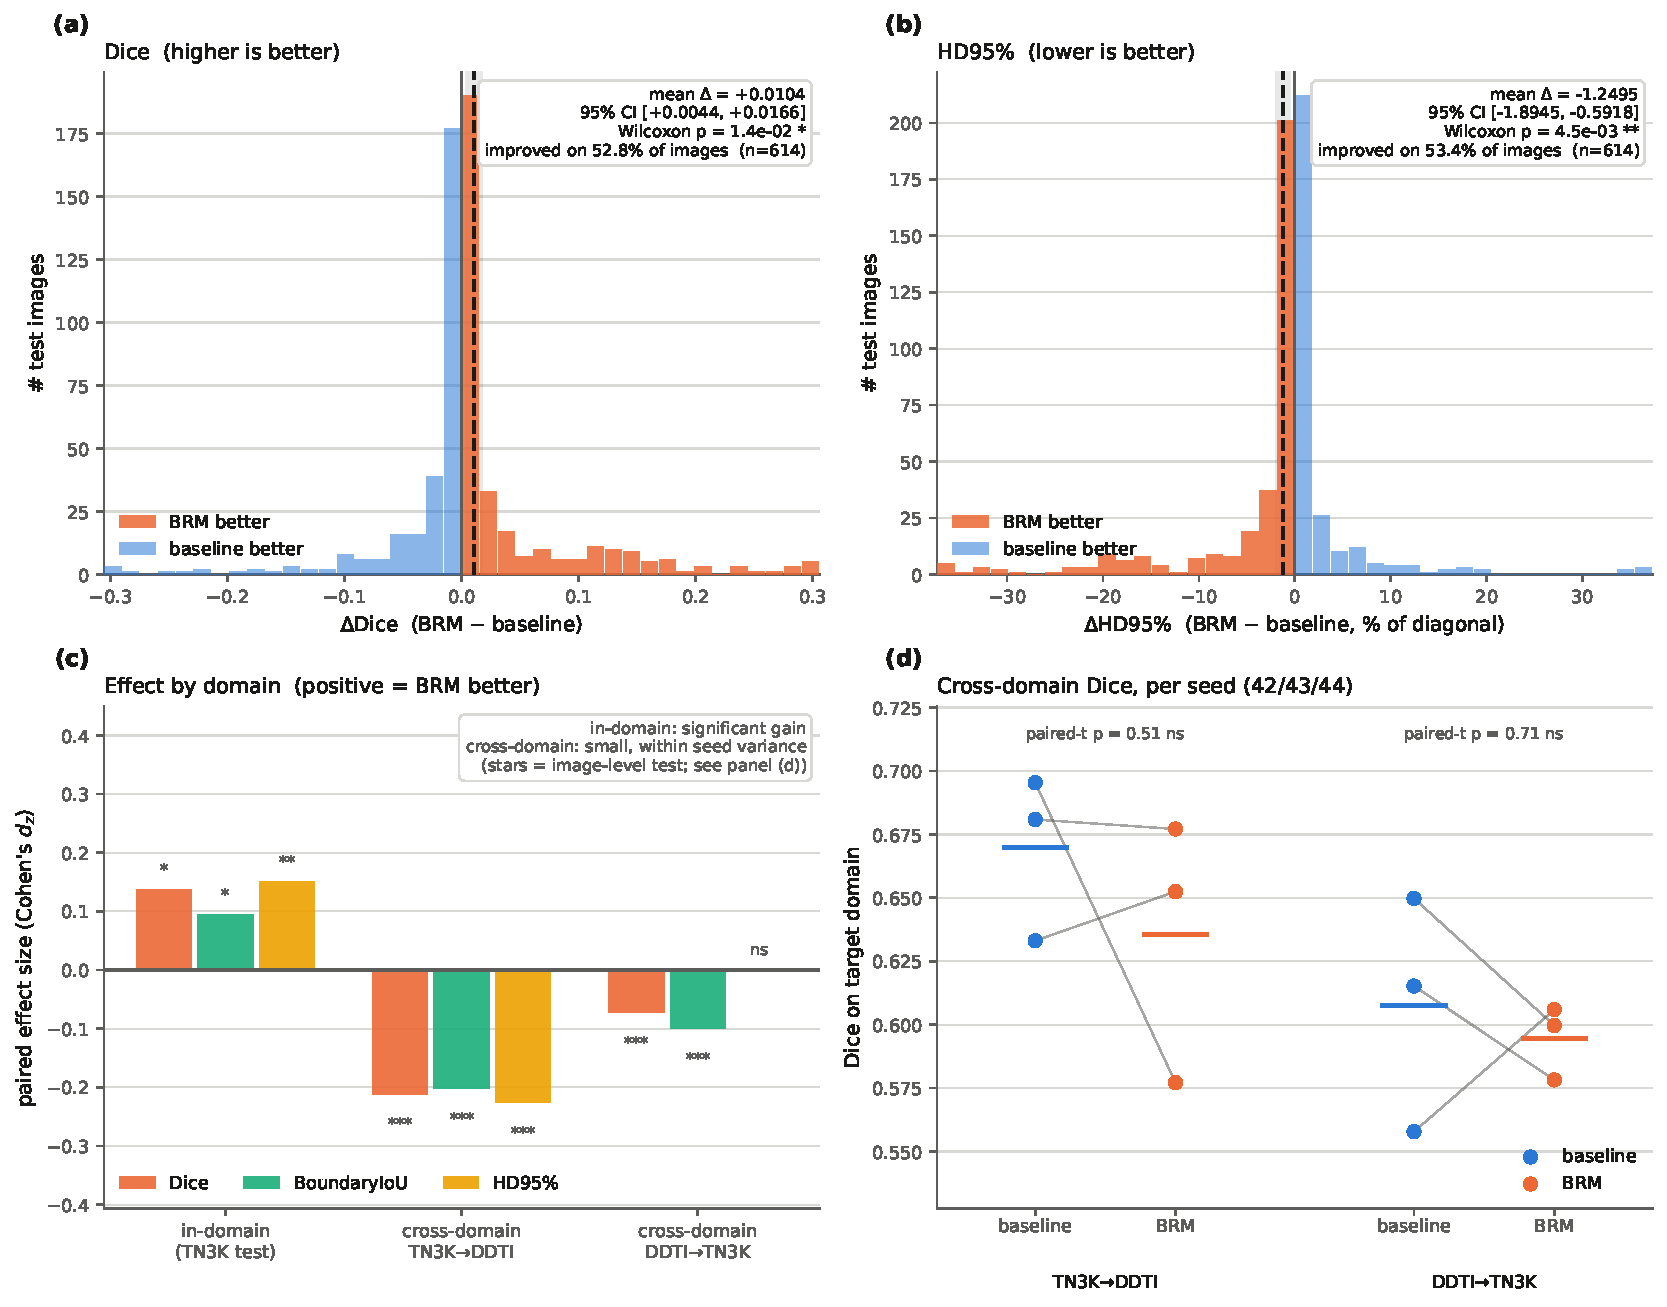
\includegraphics[width=0.97\linewidth]{fig9_significance_2x2}
  \caption[통계적 유의성과 교차 데이터셋 결과.]{통계적 유의성과 교차 데이터셋 결과. (a)(b) 영상별 대응 차이의 분포 — 점선은 평균, 회색 띠는 95\%
    신뢰구간. (c) 설정별 효과크기 $d_z$. (d) LODO 시드별 Dice — 같은 시드끼리 선으로 이었다.}
  \label{fig:significance}
\end{figure}

\paragraph{영상 단위.} 세 경계 지표 모두 유의하였다. Dice의 평균 차이는 +0.0104(95\% CI [+0.0044, +0.0166],
Wilcoxon $p$=0.014), Boundary IoU는 +0.0055([+0.0009, +0.0102], $p$=0.011), HD95는 $-$1.25\%p([$-$1.89, $-$0.59],
$p$=0.0045)였다. 세 신뢰구간 모두 0을 포함하지 않는다. 효과크기는 $d_z$=0.09--0.15로 작은 편이다.

개선 비율이 52.8--53.6\%로 절반을 조금 넘는다는 점은 해석에 중요하다. \figref{fig:significance}(a)(b)에서 보듯
대부분의 영상에서는 두 모델의 차이가 0 근처에 몰려 있고, 평균 개선은 일부 영상에서의 큰 개선에서 나온다.
즉 제안 방법은 모든 영상을 조금씩 낫게 만들기보다, 베이스라인이 경계를 크게 놓치던 일부 영상을 바로잡는 방식으로
작동한다.

\paragraph{fold 단위.} 5개 fold의 평균을 짝지은 검정에서는 세 지표 모두 유의하지 않았다(Wilcoxon $p$=0.0625,
0.1875, 0.3125). 그러나 n=5에서 양측 Wilcoxon 검정이 도달할 수 있는 최소 $p$가 0.0625이므로, Dice의 $p$=0.0625는
5개 fold가 모두 같은 방향으로 개선되었을 때 나올 수 있는 가장 강한 결과이다. 효과크기도 $d_z$=0.71--1.09로 크다.
fold 단위의 '유의하지 않음'은 효과가 없다는 증거가 아니라 표본 5개의 검정력 한계로 읽어야 한다.

이상의 결과로 \textbf{H2는 지지된다}. 경계 지표의 개선은 영상 단위에서 통계적으로 유의하고, 추론 연산량은
늘지 않았다.

\section{교차 데이터셋 일반화}\label{sec:exp_lodo}

마지막으로 제안 방법의 효과가 학습하지 않은 데이터셋에서도 유지되는지 LODO로 확인하였다(\tabref{tab:lodo}).
처음에는 시드 42 하나로 실험하였으나, 결과의 변동이 커서 시드 43, 44를 추가로 학습하여 세 시드로 반복하였다.

% 자동 생성 파일 — scripts/make_thesis.py 가 덮어쓴다. 직접 고치지 말 것.
\begin{table}[htbp]
\centering
\small
\caption[교차 데이터셋(LODO) 결과 — 3개 시드(42, 43, 44) 평균 $\pm$ 표준편차.]{교차 데이터셋(LODO) 결과 — 3개 시드(42, 43, 44) 평균 $\pm$ 표준편차. Mask mAP는 저장된 체크포인트(검증 fitness 최대 epoch)의 값이며, 경계 지표는 타깃 도메인 전체 영상에 대한 평균이다. $p$는 시드 단위 대응 $t$ 검정(n=3)이다.}
\label{tab:lodo}
\begin{adjustbox}{max width=\linewidth}
\begin{tabular}{llcccc}
\toprule
방향 & 지표 & 베이스라인 & 제안 (BRM) & $\Delta$ & 시드 단위 $p$ \\
\midrule
\multirow{4}{*}{TN3K$\rightarrow$DDTI} & Mask mAP$_{50:95}$ & 0.4465 $\pm$ 0.0136 & 0.4365 $\pm$ 0.0056 & -0.0100 & 0.454 (n.s.) \\
 & Dice & 0.6698 $\pm$ 0.0326 & 0.6356 $\pm$ 0.0521 & -0.0342 & 0.506 (n.s.) \\
 & HD95 (\%) & 21.372 $\pm$ 4.245 & 25.810 $\pm$ 7.522 & +4.438 & 0.532 (n.s.) \\
 & Boundary IoU & 0.2722 $\pm$ 0.0022 & 0.2549 $\pm$ 0.0105 & -0.0173 & 0.073 (n.s.) \\
\midrule
\multirow{4}{*}{DDTI$\rightarrow$TN3K} & Mask mAP$_{50:95}$ & 0.3146 $\pm$ 0.0210 & 0.3015 $\pm$ 0.0042 & -0.0131 & 0.444 (n.s.) \\
 & Dice & 0.6076 $\pm$ 0.0465 & 0.5946 $\pm$ 0.0145 & -0.0130 & 0.714 (n.s.) \\
 & HD95 (\%) & 23.173 $\pm$ 4.875 & 23.169 $\pm$ 1.769 & -0.004 & 0.999 (n.s.) \\
 & Boundary IoU & 0.2285 $\pm$ 0.0231 & 0.2189 $\pm$ 0.0166 & -0.0096 & 0.693 (n.s.) \\
\bottomrule
\end{tabular}
\end{adjustbox}
\end{table}


\paragraph{단일 시드의 결과.} 시드 42만 보면 TN3K$\rightarrow$DDTI에서 제안 모델의 Dice가 0.6954에서 0.5771로
0.118 떨어지고 HD95가 17.89\%에서 34.15\%로 거의 두 배가 되어, 제안 방법이 교차 데이터셋에서 크게 악화되는
것처럼 보였다(\tabref{tab:lodo_seed}). 이 차이는 637장 영상 단위 검정에서 $p<10^{-10}$으로 매우 유의하였다.

\paragraph{세 시드의 결과.} 그러나 시드를 늘리자 그림이 달라졌다. 시드 43, 44에서 제안 모델의 Dice는 0.6771,
0.6525로 베이스라인(0.6809, 0.6331)과 비슷하거나 오히려 높았고, 시드 42의 제안 모델(0.5771)이 이상치였음이
드러났다. 세 시드 평균의 차이는 TN3K$\rightarrow$DDTI에서 Dice $-$0.034, DDTI$\rightarrow$TN3K에서 $-$0.013으로
줄었고, 시드 단위 검정에서는 모든 지표가 유의하지 않았다($p$=0.073--0.999). 무엇보다 시드 간 표준편차
(Dice 기준 0.015--0.052)가 두 모델의 차이보다 크다. 즉 현재의 표본으로는 차이가 제안 방법 때문인지 실행 간
변동 때문인지 구분할 수 없다.

Mask \mAP{} 역시 두 방향 모두 제안 모델이 0.010--0.013 낮았으나 유의하지 않았다($p$=0.454, 0.444).
유일하게 일관된 신호는 TN3K$\rightarrow$DDTI의 Boundary IoU로, 세 시드 모두 제안 모델이 낮았다($\Delta$=$-$0.017,
$p$=0.073). 이 역시 유의수준에 이르지 않으므로 '약한 경향' 이상으로 해석하지 않는다.

정리하면, 경계 정교화의 효과는 학습 분포 안에서는 유의하지만 교차 데이터셋에서는 유지되지 않으며,
그렇다고 악화가 확인된 것도 아니다. \textbf{교차 데이터셋 일반화는 현재의 표본으로 판정할 수 없다}.
이 결과의 해석은 \secref{sec:disc_lodo}에서 다룬다.

\section{경량화 결과 (H3)}\label{sec:exp_quant}

\tabref{tab:quant}와 \figref{fig:quantization}은 제안 모델의 정밀도별 결과이다.

% 자동 생성 파일 — scripts/make_thesis.py 가 덮어쓴다. 직접 고치지 말 것.
\begin{table*}[htbp]
\centering
\footnotesize
\caption[정밀도별 경량화 결과 (제안 모델, held-out TN3K test, 5-fold 평균 $\pm$ 표준편차).]{정밀도별 경량화 결과 (제안 모델, held-out TN3K test, 5-fold 평균 $\pm$ 표준편차). 지연 시간은 batch 1, 640$\times$640 입력, 워밍업 15회 후 100회 평균의 fold 평균이며 fold 간 표준편차는 CPU 0.02--4.86 ms, GPU 0.05 ms 이하였다. INT8 모델의 정확도는 CPU에서 측정했다.}
\label{tab:quant}
\setlength{\tabcolsep}{3.5pt}
\begin{adjustbox}{max width=\linewidth}
\begin{tabular}{lccccccc}
\toprule
정밀도 & 크기 (MB) & CPU (ms) & GPU (ms) & Mask mAP$_{50:95}$ & Dice & HD95 (\%) & BIoU \\
\midrule
PyTorch FP32 & 6.01 & -- & -- & 0.6267 $\pm$ 0.0081 & 0.8300 $\pm$ 0.0039 & 8.378 $\pm$ 0.775 & 0.4414 $\pm$ 0.0050 \\
ONNX FP32 & 11.63 & 62.82 & 3.53 & 0.6188 $\pm$ 0.0077 & 0.8300 $\pm$ 0.0049 & 8.529 $\pm$ 0.899 & 0.4402 $\pm$ 0.0056 \\
ONNX FP16 & 5.87 & -- & 3.13 & 0.6194 $\pm$ 0.0080 & 0.8301 $\pm$ 0.0050 & 8.516 $\pm$ 0.911 & 0.4403 $\pm$ 0.0058 \\
ONNX Runtime INT8 & 5.45 & 44.00 & -- & 0.6032 $\pm$ 0.0160 & 0.8184 $\pm$ 0.0123 & 9.395 $\pm$ 1.026 & 0.4299 $\pm$ 0.0121 \\
\textbf{OpenVINO INT8} & \textbf{3.71} & \textbf{4.10} & \textbf{--} & \textbf{0.6161 $\pm$ 0.0085} & \textbf{0.8290 $\pm$ 0.0051} & \textbf{8.497 $\pm$ 0.706} & \textbf{0.4379 $\pm$ 0.0075} \\
\bottomrule
\end{tabular}
\end{adjustbox}
\end{table*}


\begin{figure}[htbp]
  \centering
  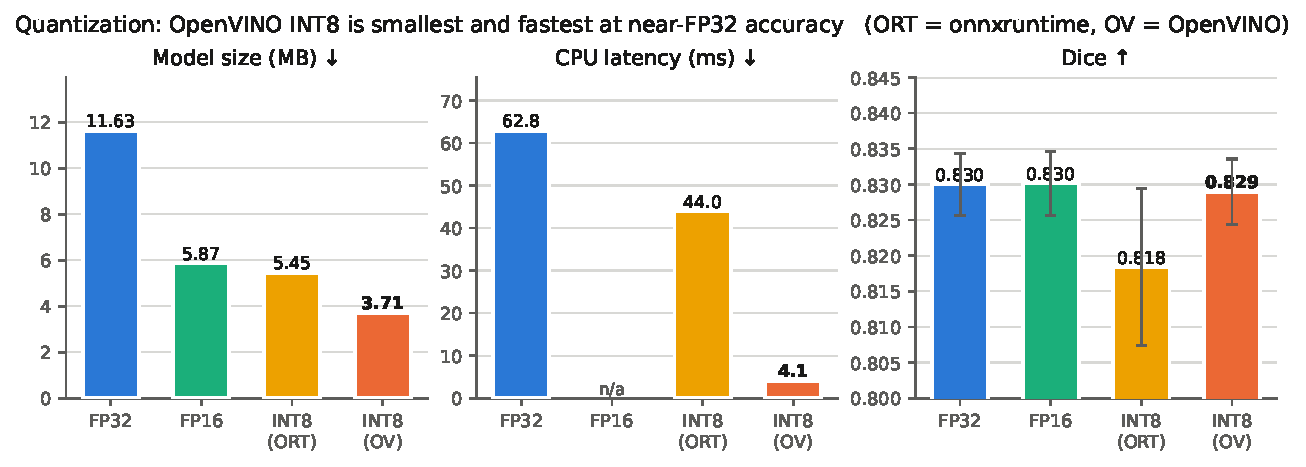
\includegraphics[width=\linewidth]{fig3_quantization}
  \caption[정밀도별 모델 크기, CPU 지연, Dice.]{정밀도별 모델 크기, CPU 지연, Dice. ORT = ONNX Runtime, OV = OpenVINO.}
  \label{fig:quantization}
\end{figure}

\paragraph{FP32와 FP16.} ONNX FP32는 Dice 0.8300으로 PyTorch와 같았고, Mask \mAP{}는 0.6188로 0.008 낮았다.
경계 지표가 그대로라는 점에서 마스크 자체의 품질보다는 검증 절차에서 ONNX 예측을 처리하는 방식의 차이일 가능성이
있으나, 원인은 확인하지 못하였다. FP16은 FP32와 정확도가 같으면서 크기가
절반(5.87 MB)이고 GPU 지연이 3.53 ms에서 3.13 ms로 줄어, GPU 배포에서는 손실 없는 선택이다.

\paragraph{INT8.} 두 INT8 경로의 결과는 크게 달랐다. ONNX Runtime INT8은 CPU 지연이 44.00 ms로 FP32(62.82 ms)보다
30\% 빨라지는 데 그쳤고, 정확도도 Mask \mAP{} 0.6032, Dice 0.8184로 가장 많이 떨어졌다. 반면 OpenVINO INT8은
3.71 MB로 가장 작으면서 CPU 지연 4.10 ms로 FP32보다 15.3배, ONNX Runtime INT8보다 10.7배 빨랐다.
정확도 손실은 Dice 0.001, Mask \mAP{} 0.003(ONNX FP32 대비)에 그쳤고 HD95는 8.497\%로 오히려 FP32(8.529\%)보다
조금 나았다. fold 간 지연의 표준편차도 0.02 ms로 가장 안정적이었다.

\figref{fig:pareto}는 정확도와 CPU 지연의 절충을 한눈에 보여 준다. OpenVINO INT8은 지연, 크기, 정확도 모두에서
다른 CPU 후보를 앞서는 지배적 선택이다.

\begin{figure}[htbp]
  \centering
  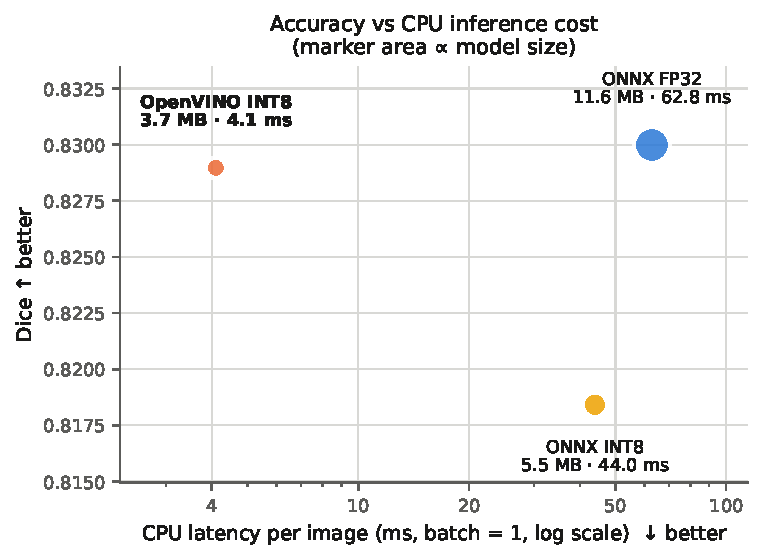
\includegraphics[width=0.62\linewidth]{fig2_accuracy_vs_latency}
  \caption[CPU 지연과 Dice의 절충.]{CPU 지연과 Dice의 절충. 마커 넓이는 모델 파일 크기에 비례한다. 가로축은 로그 척도이다.}
  \label{fig:pareto}
\end{figure}

OpenVINO INT8은 CPU에서 영상 한 장을 4.10 ms에 처리하므로 순전파만으로는 초당 약 240장을 처리할 수 있으며, Dice 손실은
fold 표준편차(0.005)보다 작다. 따라서 \textbf{H3은 OpenVINO INT8 경로에서 지지된다}. ONNX Runtime INT8 경로는
지연과 정확도 모두에서 기준에 미치지 못하므로, 같은 'INT8 사후 양자화'라도 변환 도구에 따라 결론이 달라진다는
점을 함께 밝혀 둔다.

\section{단계별 누적 결과}\label{sec:exp_final}

\tabref{tab:final}은 베이스라인에서 최종 배포 모델까지의 누적 변화이다.

% 자동 생성 파일 — scripts/make_thesis.py 가 덮어쓴다. 직접 고치지 말 것.
\begin{table*}[htbp]
\centering
\footnotesize
\caption[단계별 누적 결과 (held-out TN3K test, 5-fold 평균).]{단계별 누적 결과 (held-out TN3K test, 5-fold 평균). PyTorch 모델의 지연 시간은 배포 형식과 측정 조건이 달라 비교에서 제외했다.}
\label{tab:final}
\begin{adjustbox}{max width=\linewidth}
\begin{tabular}{lccccccc}
\toprule
모델 & Mask mAP$_{50:95}$ & Dice & HD95 (\%) & BIoU & 크기 (MB) & CPU (ms) & GPU (ms) \\
\midrule
베이스라인 nano & 0.6272 & 0.8195 & 9.628 & 0.4358 & 6.00 & -- & -- \\
+ 경계 정교화 & 0.6267 & 0.8300 & 8.378 & 0.4414 & 6.01 & -- & -- \\
+ ONNX FP16 & 0.6194 & 0.8301 & 8.516 & 0.4403 & 5.87 & -- & 3.13 \\
+ ONNX Runtime INT8 & 0.6032 & 0.8184 & 9.395 & 0.4299 & 5.45 & 44.00 & -- \\
\textbf{+ OpenVINO INT8 (최종)} & \textbf{0.6161} & \textbf{0.8290} & \textbf{8.497} & \textbf{0.4379} & \textbf{3.71} & \textbf{4.10} & \textbf{--} \\
\bottomrule
\end{tabular}
\end{adjustbox}
\end{table*}


경계 정교화로 얻은 개선은 양자화를 거친 뒤에도 대부분 유지되었다. 최종 OpenVINO INT8 모델은 베이스라인
PyTorch 모델과 비교하여 Dice +0.0095(0.8195$\rightarrow$0.8290), HD95 $-$11.7\%(9.628$\rightarrow$8.497),
Boundary IoU +0.0021을 유지하면서, 파일 크기는 6.00 MB에서 3.71 MB로 줄고 CPU에서 4.10 ms에 동작한다.
Mask \mAP{}는 0.6272에서 0.6161로 0.011 낮아졌는데, 대부분 PyTorch에서 ONNX로 바꿀 때 생긴 차이(0.008)이다.
